% Copyright 2004 by Till Tantau <tantau@users.sourceforge.net>.
%
% In principle, this file can be redistributed and/or modified under
% the terms of the GNU Public License, version 2.
%
% However, this file is supposed to be a template to be modified
% for your own needs. For this reason, if you use this file as a
% template and not specifically distribute it as part of a another
% package/program, I grant the extra permission to freely copy and
% modify this file as you see fit and even to delete this copyright
% notice. 

\documentclass{beamer}

% There are many different themes available for Beamer. A comprehensive
% list with examples is given here:
% http://deic.uab.es/~iblanes/beamer_gallery/index_by_theme.html
% You can uncomment the themes below if you would like to use a different
% one:
%\usetheme{AnnArbor}
%\usetheme{Antibes}
%\usetheme{Bergen}
%\usetheme{Berkeley}
%\usetheme{Berlin}
%\usetheme{Boadilla}
%\usetheme{boxes}
%\usetheme{CambridgeUS}
%\usetheme{Copenhagen}
%\usetheme{Darmstadt}
\usetheme{default}
%\usetheme{Frankfurt}
%\usetheme{Goettingen}
%\usetheme{Hannover}
%\usetheme{Ilmenau}
%\usetheme{JuanLesPins}
%\usetheme{Luebeck}
%\usetheme{Madrid}
%\usetheme{Malmoe}
%\usetheme{Marburg}
%\usetheme{Montpellier}
%\usetheme{PaloAlto}
%\usetheme{Pittsburgh}
%\usetheme{Rochester}
%\usetheme{Singapore}
%\usetheme{Szeged}
%\usetheme{Warsaw}

\usepackage{amsmath}
\setbeamercovered{transparent}

\usepackage{pifont}% http://ctan.org/pkg/pifont
\newcommand{\cmark}{\ding{51}}%
\newcommand{\xmark}{\ding{55}}%

\usepackage[many]{tcolorbox}
\newtcolorbox{cross}{blank,breakable,parbox=false,
  overlay={\draw[red,line width=1pt] (interior.south west)--(interior.north east);
    \draw[red,line width=1pt] (interior.north west)--(interior.south east);}}

\title{Anomaly detection based on generative adversarial networks for new physics mining at the LHC}

\author{Oliver Knapp \inst{1}}
% - Give the names in the same order as the appear in the paper.
% - Use the \inst{?} command only if the authors have different
%   affiliation.

\institute[Swiss Federal Institute of Technology] % (optional, but mostly needed)
{
  \inst{1}%
  Department of Physics \\
  Swiss Federal Institute of Technology
}
% - Use the \inst command only if there are several affiliations.
% - Keep it simple, no one is interested in your street address.

\date{Semester Project Presentation, 2019}
% - Either use conference name or its abbreviation.
% - Not really informative to the audience, more for people (including
%   yourself) who are reading the slides online

\subject{High Energy Physics}
% This is only inserted into the PDF information catalog. Can be left
% out. 

% If you have a file called "university-logo-filename.xxx", where xxx
% is a graphic format that can be processed by latex or pdflatex,
% resp., then you can add a logo as follows:

% \pgfdeclareimage[height=0.5cm]{university-logo}{university-logo-filename}
% \logo{\pgfuseimage{university-logo}}

% Delete this, if you do not want the table of contents to pop up at
% the beginning of each subsection:
\AtBeginSection[]
{
  \begin{frame}<beamer>{Outline}
    \tableofcontents[currentsection,currentsubsection]
  \end{frame}
}
\AtBeginSubsection[]
{
  \begin{frame}<beamer>{Outline}
    \tableofcontents[currentsection,currentsubsection]
  \end{frame}
}

% Let's get started
\begin{document}

\begin{frame}
  \titlepage
\end{frame}

\begin{frame}{Outline}
  \tableofcontents
  % You might wish to add the option [pausesections]
\end{frame}

% Section and subsections will appear in the presentation overview
% and table of contents.
\section{Introduction}

\begin{frame}{Overview}
  \begin{itemize}
      \item Main goal of LHC: search for deviations from the SM \pause
      \item Typically fully-supervised hypothesis tests (model-dependent) \pause
      \item Alternative: model-independent searches \pause
      \item Cerri et al. proposed anomaly detection using variational autoencoders (VAE) to implement this task \pause
      \item We investigate a GAN based anomaly detector and
      \begin{itemize}
        \pause
        \item benchmark and compare it with VAE
        \pause
        \item demonstrate its effectiveness for offline analysis by simulating a rediscovery of the top quark
      \end{itemize}
  \end{itemize}
\end{frame}

\begin{frame}{Anomaly detection based BSM search}
  \begin{itemize}
      \item<1-> It is expected that BSM events are much rarer compared to SM events $\implies$ Try to isolate rare events (outliers)
      \item<2-> This task belongs to the field of anomaly detection (AD), which can be divided into three categories:
      \begin{itemize}
        \item<3-> Supervised AD $\rightarrow$ requires labeling samples as "normal" or "anomalous" \uncover<4->{\textcolor{red}{\xmark}}
        \item<5-> Semi-supervised AD $\rightarrow$ training set must only contain "normal" samples \uncover<6->{\textcolor{red}{\xmark}}
        \item<7-> Unsupervised AD $\rightarrow$ training set mostly consists of "normal" samples but may contain a small fraction of "anomalous" samples \uncover<8->{\textcolor{green}{\cmark}}
      \end{itemize}
  \end{itemize}
\end{frame}

\section{GAN based anomaly detection}

\begin{frame}{Motivating generative adversarial networks}
  \begin{itemize}
      \item<1-> Generative adversarial networks (GANs) have recently been very successful
      \item<2-> Similar to VAE (used by Cerri et al.)
      \item<3-> Both GAN and VAE aim to learn the training set distribution
  \end{itemize}
\end{frame}

\begin{frame}{Generative adversarial networks}
  \begin{itemize}
      \item<1-> Basic idea: two networks compete against each other
      \item<2-> Generator network $G: \mathcal{Z} \rightarrow \mathcal{X}$ learns to generate new samples resembling the training set
      \item<3-> Discriminator network $D:\mathcal{X} \rightarrow [0,1]$ learns to distinguish real samples from the generated ones
      \item<4-> Training = solving saddle point problem
      \begin{equation}
      \underset{G}{\textup{min}}\, \underset{D}{\textup{max}}\, V(D,G),
      \end{equation}
      where
      \begin{equation}
        V(D,G)=\mathbb{E}_{x\sim p_\mathcal{X}}[log\,D(x)] + \mathbb{E}_{z\sim p_\mathcal{Z}}[log\,(1-D(G(z))]
      \end{equation}
      
      \item<5-> Solution has property $p_\mathcal{X}=p_G$
  \end{itemize}
\end{frame}

\begin{frame}{GAN for anomaly detection}
  \begin{itemize}
      \item<1-> Exploit $p_\mathcal{X}\approx p_G$ (after training)
      \item<2-> $\textup{Prob[x \textup{is normal sample}]}\sim p_\mathcal{X}(x) \approx p_G(x)$
      \item<3-> Problem: $p_G$ is not given explicitly, but can only be sampled from by taking $G(z)$ ($z$ uniformly sampled from latent space $\mathcal{Z}$)
      \item<4-> Instead, we adopt a reconstruction based strategy similar to VAE:
      \begin{equation}
        A(x) \sim \underset{z}{\textup{min}} \; \textup{Loss}_{\textup{reco}}(x, G(z))
      \end{equation}
      \item<5-> Solving the minimization problem (e.g. with gradient descent) is computationally very expensive
  \end{itemize}
\end{frame}

\begin{frame}{ALAD algorithm}
  \begin{itemize}
      \item<1-> Zenati et al. propose to use bidirectional-GANs (BiGAN)
      \item<2-> An encoder network $E: \mathcal{X} \rightarrow \mathcal{Z}$ is simultaneously trained with the generator
      \item<3-> The objective of the encoder is to approximate the inverse of the generator, i.e. $G(E(x))\approx x$
      \item<4-> Achieved by solving the saddle point problem
      \begin{align}
    \underset{G,E}{\textup{min}}\, \underset{D_{xz}}{\textup{max}}\, V(D_{xz},E,G),
\end{align}
with the value function given as
\begin{equation}
\begin{split}
    V(D_{xz},E,G)=& \mathbb{E}_{x\sim p_\mathcal{X}}[log\,D_{xz}(x, E(x))] + \\
    & \mathbb{E}_{z\sim p_\mathcal{Z}}[log\,(1-D_{xz}(G(z), z)]
\end{split}
\end{equation}
  \end{itemize}
\end{frame}

\begin{frame}{ALAD algorithm}
  \begin{itemize}
      \item<1-> Training process does not necessarily converge $\rightarrow$ further modifications needed.
      \item<2-> Add discriminator $D_{xx}$ to enforce cycle consistency $G(E(x))\approx x$
      \item<3-> Add discriminator $D_{zz}$ to regularize latent space
  \end{itemize}
  \begin{figure}[]
    \begin{center}
    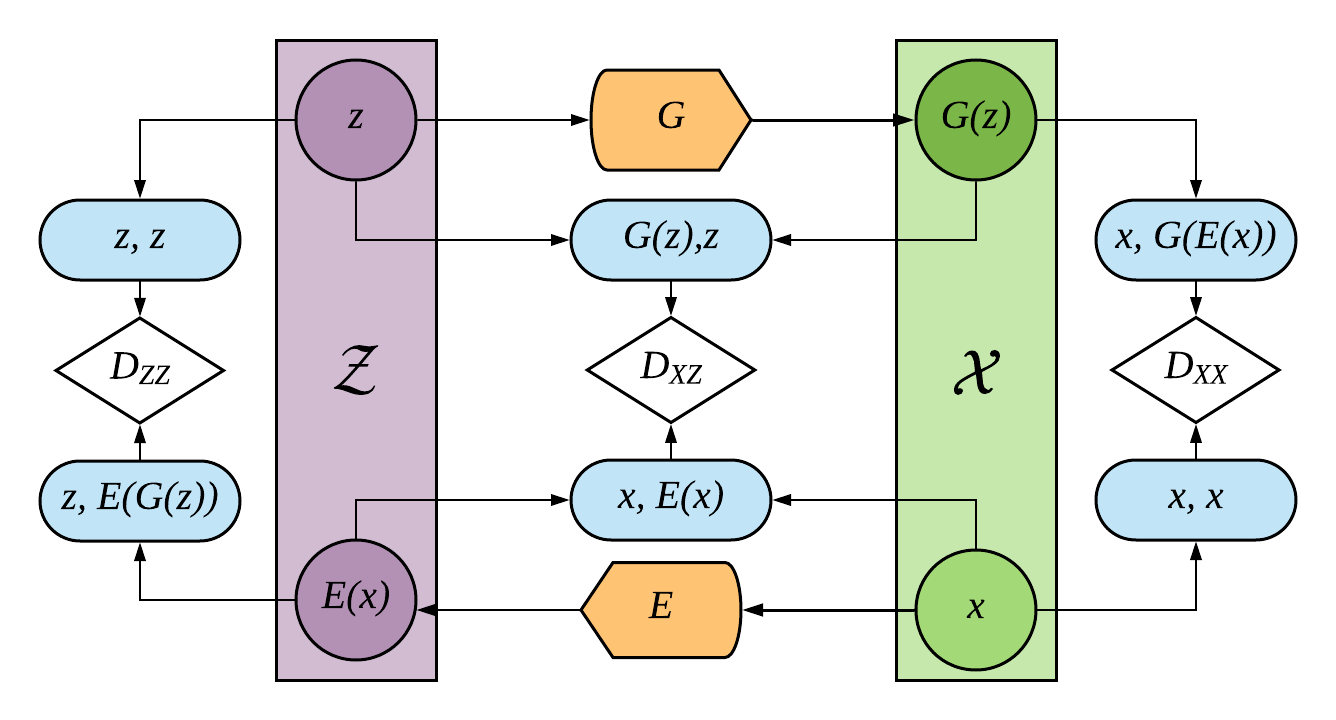
\includegraphics[width=0.7\textwidth]{dladded}
    \caption{Adapted from "Adversarially learned anomaly detection" by Zenati et al.}
    \label{fig:alad}
    \end{center}
  \end{figure}
\end{frame}

\begin{frame}{ALAD anomaly scores}
  \begin{itemize}
      \item<1-> Four proposed anomaly score models
      \item<2-> $L_1$-score: $A(x)=||x-G(E(x))||_{1}$
      \item<3-> $L_2$-score: $A(x)=||x-G(E(x))||_{2}$
      \item<4-> Logits-score: $A(x)=log(D_{xx}(x, G(E(x)))$
      \item<5-> Features-score: $A(x)=||f_{xx}(x,x) - f_{xx}(x, G(E(x)))||_1$, where $f_{xx}(\cdot,\cdot)$ are the activation values in the last hidden layer of $D_{xx}$
  \end{itemize}
\end{frame}

\begin{frame}{Data format}
  \begin{itemize}
      \item<1-> One event recorded by the CMS detector contains $O(10^3)$ particles resulting in $O(10^4)$ parameters
      \item<2-> To reduce dimensionality an event is represented with high-level-features (HLF)
      \item<3-> Jet quantities: $H_T$, $M_J$, $N_J$, $N_b$
      \item<4-> Muon/electron quantities: $p_{T,TOT}^\mu$, $M_\mu$, $N_\mu$, $p_{T,TOT}^e$, $M_e$, $N_e$
      \item<5-> Particle multiplicities: $N_{neu}$, $N_{ch}$, $N_\gamma$
      \item<6-> Missing transverse momentum $p_T^\textup{miss}$
      \item<7-> Selected lepton $\ell$ quantities: $p_T^\ell$, $\eta_\ell$, $q_\ell$, $\textup{IsEle}$, $\textup{Iso}_{ch}^\ell$, $\textup{Iso}_{neu}^\ell$, $\textup{Iso}_{\gamma}^\ell$
      \item<8-> Selected lepton and missing system: $M_T$, $p_{T,\parallel}^\textup{miss}$, $p_{T,\perp}^\textup{miss}$
  \end{itemize}
\end{frame}

\section{Benchmark}

\begin{frame}{Benchmark setup}
  \begin{itemize}
      \item<1-> Goal: Measure ALAD's efficiency in discriminating BSM from SM events
      \item<2-> Train ALAD on pure SM samples
      \item<3-> Run trained model on a mixture of SM and BSM samples
      \item<4-> From the anomaly scores we calculate evaluation metrics like ROC and $\textup{LR}_+$
  \end{itemize}
\end{frame}

\begin{frame}{Benchmark datasets}
  \begin{itemize}
      \item<1-> Benchmark datasets were provided by Cerri et al. (used to evaluate VAE)
      \item<2-> Events were generated with \texttt{PYTHIA8} at $\sqrt{s}=13$~TeV
      \item<3-> Dataset includes four most relevant SM processes:
        \begin{itemize}
            \item<4-> Inclusive W production: $W \rightarrow \ell\nu$
            \item<5-> Inclusive Z production: $Z \rightarrow \ell\ell$
            \item<6-> QCD multijet production
            \item<7-> $t\Bar{t}$ production
        \end{itemize}
      \item<8-> and four BSM processes:
      \begin{itemize}
    \item<9-> $LQ\rightarrow b\tau$ (LQ=leptoquark with mass 80~GeV)
    \item<10-> $A \rightarrow 4\ell$ (A=neutral scalar boson with mass 50~GeV)
    \item<11-> $h^0 \rightarrow \tau\tau$ ($h^0$=neutral scalar boson with mass 60~GeV)
    \item<12-> $h^\pm \rightarrow \tau\nu$ ($h^\pm$=charged scalar boson with mass 60~GeV)
\end{itemize}
  \end{itemize}
\end{frame}

\begin{frame}{Benchmark results}{Receiver operating characteristic (ROC)}
\begin{figure}[!htb]
\centering
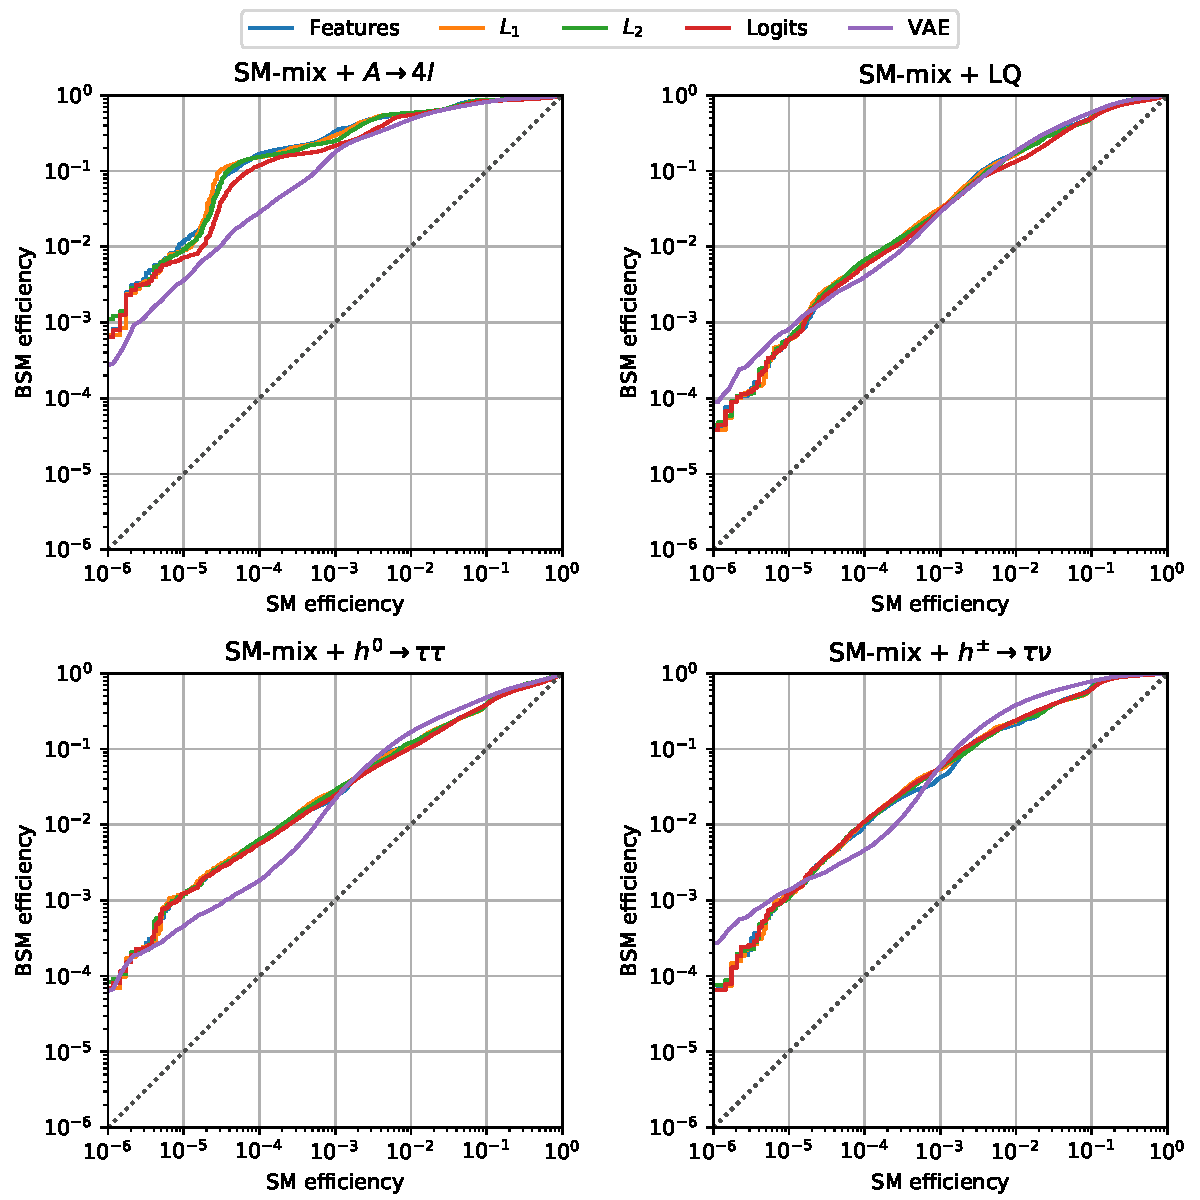
\includegraphics[width=0.7\textwidth]{roc.pdf}
\end{figure}
\end{frame}

\begin{frame}{Benchmark results}{ROC and $\textup{LR}_+$ for the $L_1$ score}
  \begin{itemize}
      \item<1-> Positive likelihood ratio $\textup{LR}_+ = \frac{\textup{TPR}}{\textup{FPR}}$
  \end{itemize}
\begin{figure}[!htb]
\centering
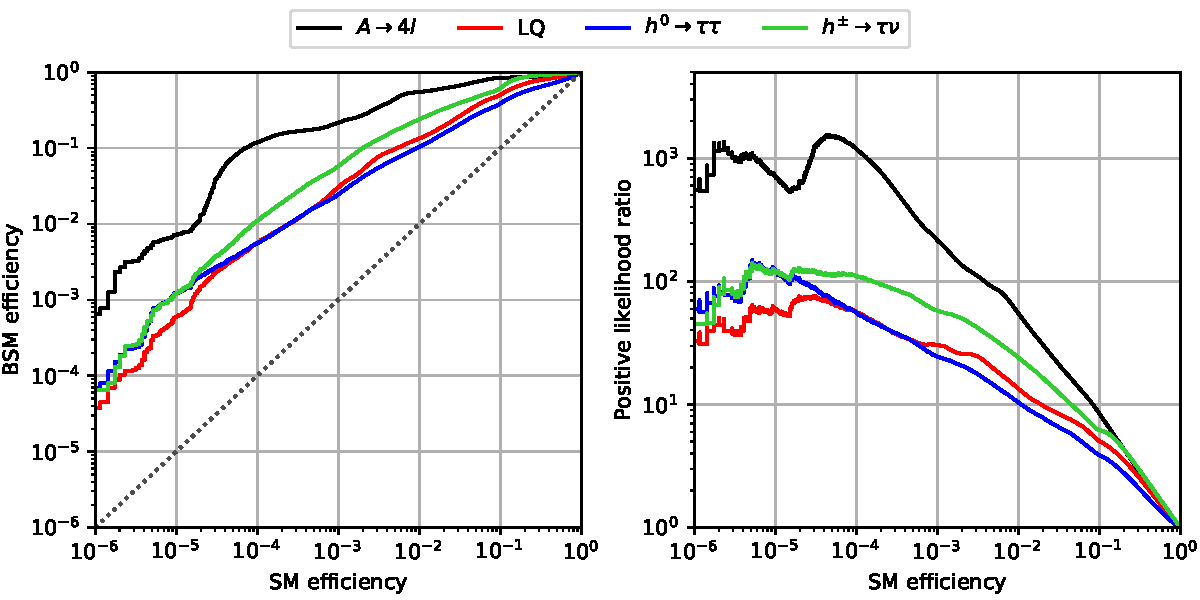
\includegraphics[width=1\textwidth]{roc_lrp.pdf}
\end{figure}
\end{frame}

\begin{frame}{Benchmark results}{$L_1$ score distribution}
\begin{figure}[!htb]
\centering
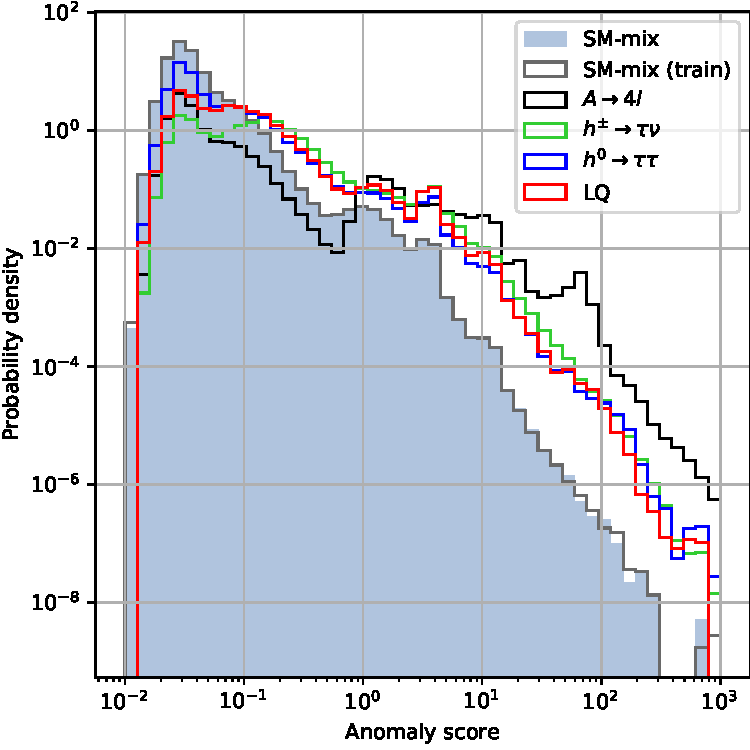
\includegraphics[width=0.7\textwidth]{score_dist.pdf}
\end{figure}
\end{frame}

\begin{frame}{Benchmark conclusion}
  \begin{itemize}
      \item<1-> ALAD has shown a performance at least comparable to VAE 
      \item<2-> ALAD's model is generic while the VAE used by Cerri et al. has customized loss function for each HLF quantity
      \item<3-> This flexibility could prove if a customized set of input quantities is desired (e.g. for certain BSM scenarios)
  \end{itemize}
\end{frame}

\section{Top quark rediscovery}

\begin{frame}{Overview}
  \begin{itemize}
      \item<1-> Benchmark only investigated semi-supervised problem
      \item<2-> Cerri et al. indirectly demonstrated that VAE can be trained on data
      \item<3-> They propose to employ anomaly detection in the trigger system
      \item<4-> We present an anomaly detection based model-independent offline analysis strategy
      \item<5-> We demonstrate the effectiveness of this strategy by simulating a rediscovery of the top quark
      \item<6-> From now on let's assume the existence of top quark is neither experimentally nor theoretically established
  \end{itemize}
\end{frame}

\subsection{Offline analysis}

\begin{frame}{Strategy}
  \begin{itemize}
      \item<1-> Model background processes (SM without top) with MC simulation
      \item<2-> Run ALAD on both data and MC background
      \item<3-> Expectation: Anomaly selection amplifies signal events in data $\implies$ easier to detect discrepancy
  \end{itemize}
\end{frame}

\begin{frame}{Data description}
  \begin{itemize}
      \item<1-> data = \textit{SingleMu primary dataset from RunB of 2012} ($\int\!L = 4.429\,\textup{fb}^{-1}$)
      \item<2-> Background modeling:
      \begin{itemize}
          \item<3-> Exclusive W production with 1, 2 or 3 jets: $pp \rightarrow W+\textup{Jets} \rightarrow \ell\nu$
          \item<4-> Exclusive Drell-Yan process with 1, 2, 3 or 4 jets: $pp \rightarrow Z/\gamma^* + \textup{Jets} \rightarrow \ell\ell$
      \end{itemize}
  \end{itemize}
\uncover<5->{
  \begin{table}[]
\centering
\begin{tabular}{l|r|r}
\hline
Process   & $\sigma$ [pb] & K-factor \\ \hline
$W$ + 1Jet    & 4480         & 1.23 \\
$W$ + 2Jets   & 1435         & 1.23 \\
$W$ + 3Jets   & 304          & 1.23 \\
$Z$/$\gamma^*$ + 1Jet  & 561     & 1.23 \\
$Z$/$\gamma^*$ + 2Jets   & 181     & 1.23 \\
$Z$/$\gamma^*$ + 3Jets   & 51     & 1.23 \\
$Z$/$\gamma^*$ + 4Jets   & 15     & 1.23 \\
$t\bar{t}$ + Jets        & 164  & 1.66 \\
\hline
\end{tabular}
\caption{LO cross section at $\sqrt{s}=8$~TeV for background processes.}
\label{table:mc-datasets}
\end{table}}
  
\end{frame}

\begin{frame}{Preprocessing}
  \begin{itemize}
      \item<1-> Wrote Python script to converted AOD data files to HLF quantities (converted $O(100)$~TB of data)
      \item<2-> Most dominant processes not modeled: QCD, $pp \rightarrow W$ and $pp \rightarrow Z/\gamma^*$
      \item<3-> Need preselection: 
      \begin{itemize}
          \item<4-> $p_T>23$~GeV, $\left | \eta \right | < 1.4$ and $\text{Iso}<\textup{0.1}$ to remove QCD
          \item<5-> $N_J\geq 2$ to remove $pp \rightarrow W$ and $pp \rightarrow Z/\gamma^*$
      \end{itemize}
  \end{itemize}
\end{frame}

\begin{frame}{Anomaly selection}
  \begin{itemize}
      \item<1-> Event is considered anomalous $\iff$ $L_1$ anomaly score exceeds fixed threshold
      \item<2-> Threshold is set s.t. the fraction of selected events is $O(10^{-3})$ 
  \end{itemize}
\end{frame}

\begin{frame}{Anomaly selection results}
\begin{columns}
\begin{column}{0.5\textwidth}
    \begin{center}
     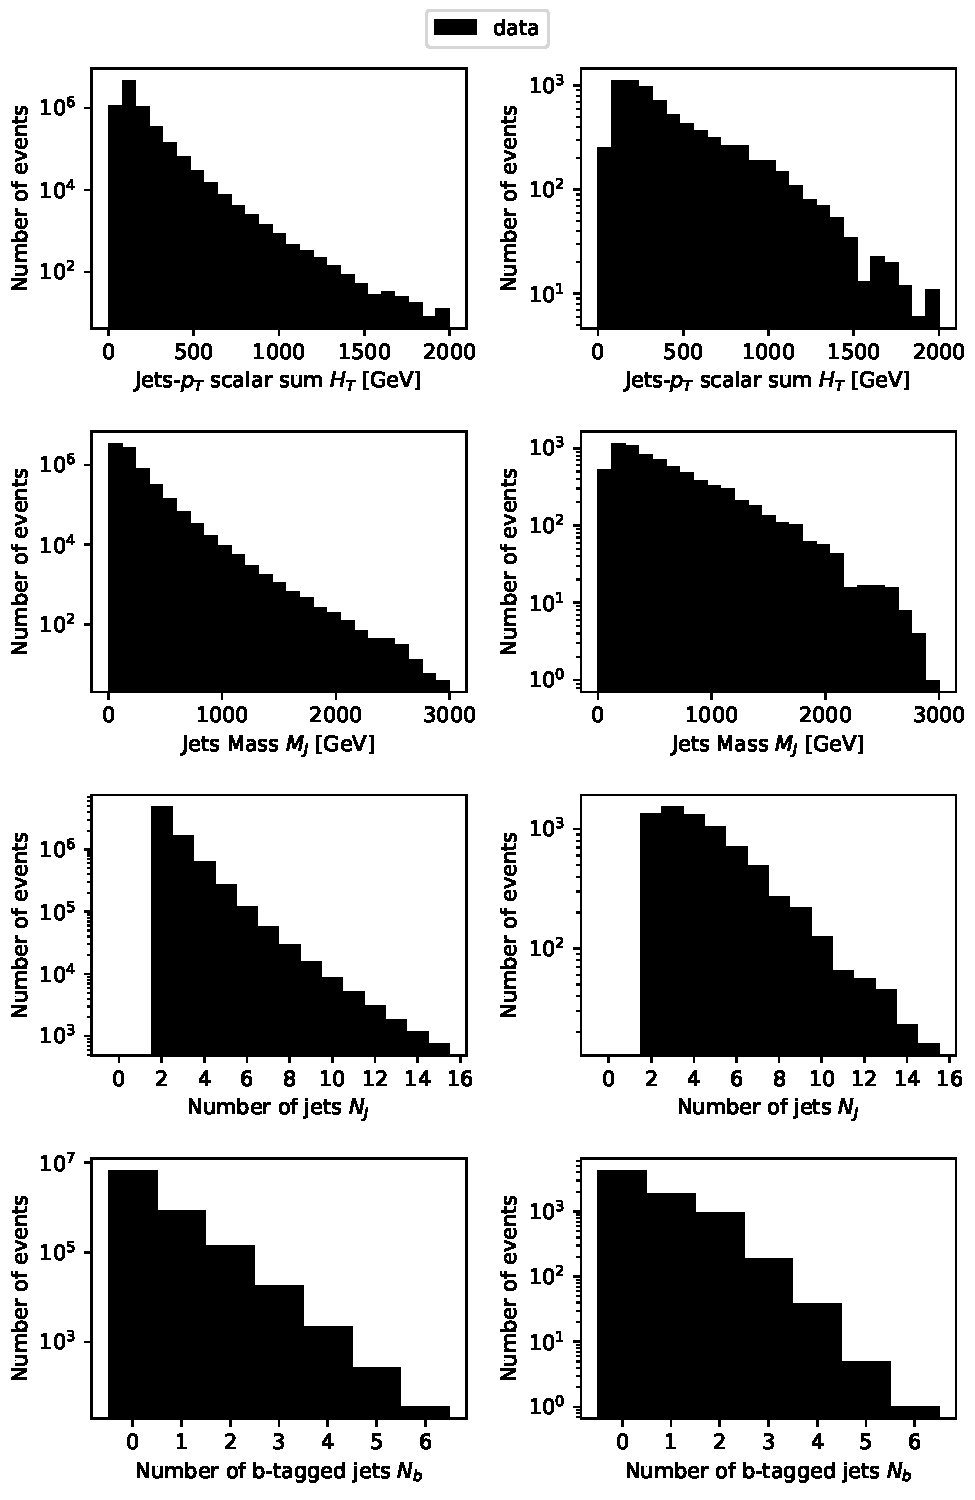
\includegraphics[width=1\textwidth]{data.pdf}
     \end{center}
\end{column}
\begin{column}{0.5\textwidth}  %%<--- here
    \begin{center}
     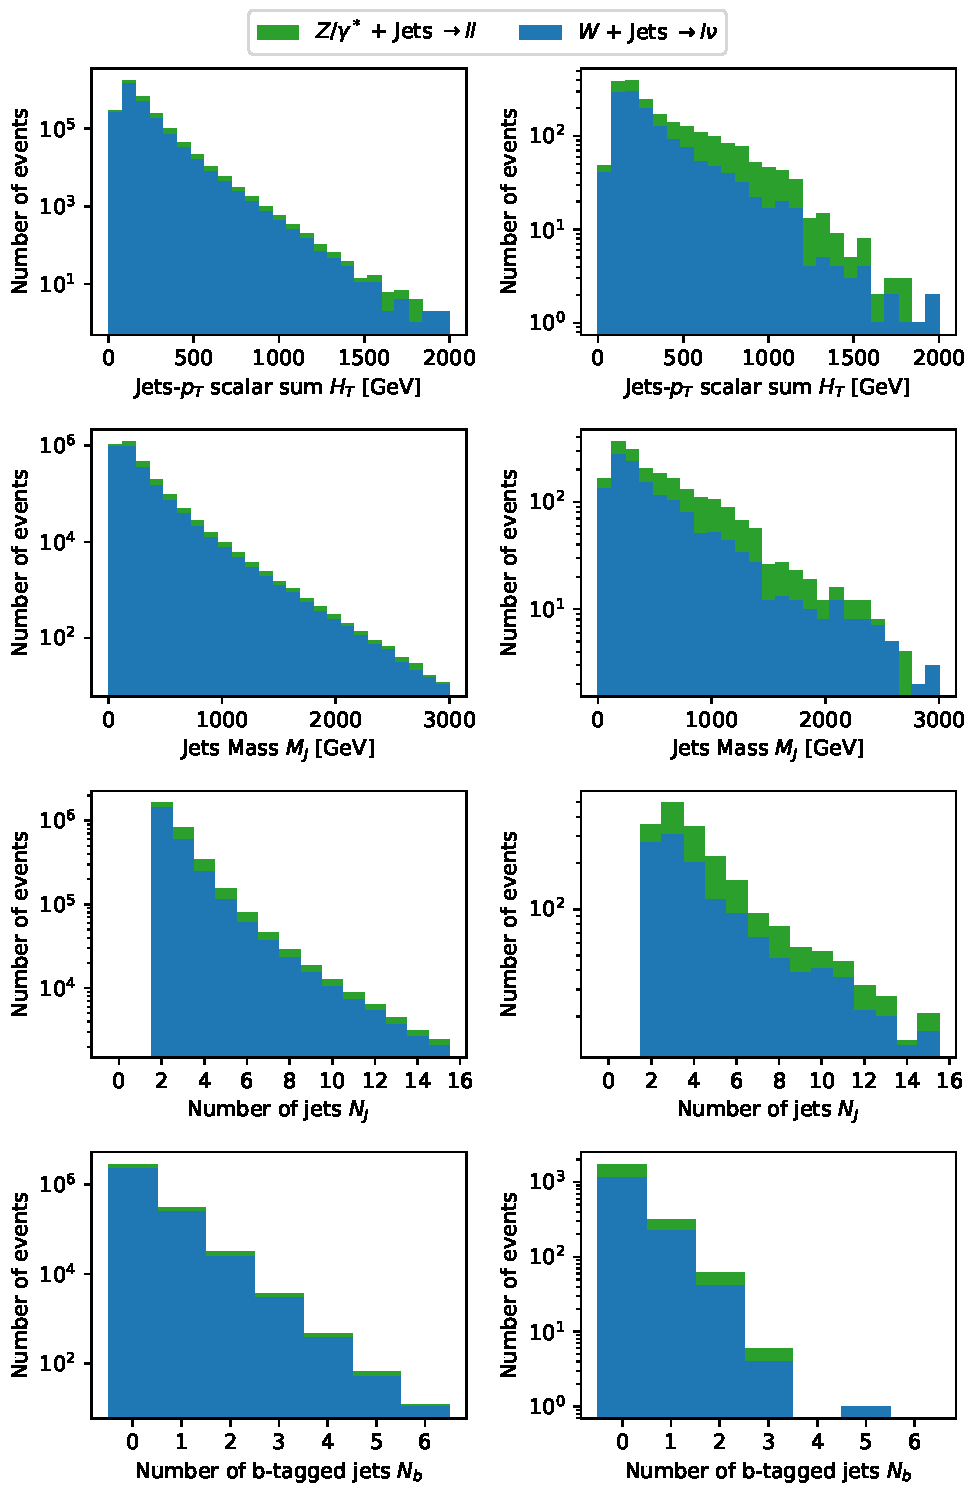
\includegraphics[width=1\textwidth]{mc_b.pdf}
     \end{center}
\end{column}
\end{columns}
\end{frame}

\begin{frame}{Anomaly selection transfer function}
  \begin{itemize}
      \item<1-> One can see with the naked eye a difference in the b-tagged jets $N_b$
      \item<2-> Cannot directly compare data with MC in joint plot
      \item<3-> Instead we propose to consider (what we call) the anomaly selection transfer function (ASTF)
      \begin{equation}
      \textup{ASTF}(q) = \frac{\textup{PDF}_{\textup{AS}}(q)}{\textup{PDF}_{0}(q)},
      \end{equation}
      \item<4-> The ASTF gives the anomaly selection acceptance rate per bin
  \end{itemize}
\end{frame}

\begin{frame}{Anomaly selection transfer function}
    \begin{center}
     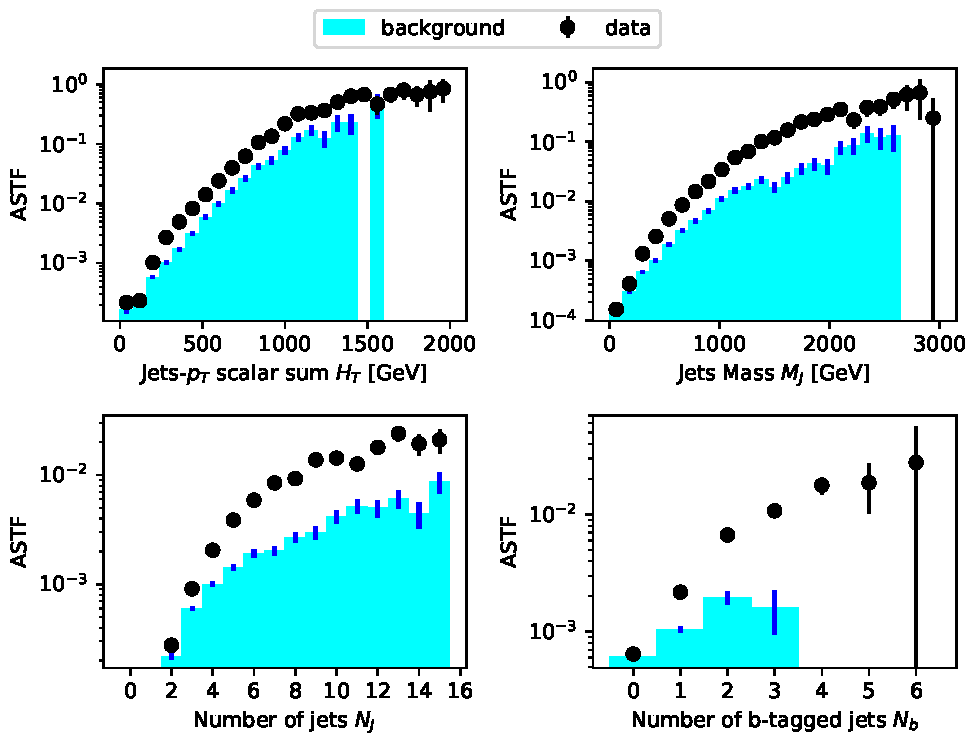
\includegraphics[width=1\textwidth]{astf.pdf}
    \end{center}
\end{frame}

\begin{frame}{Postselection}
\begin{itemize}
    \item<1-> After anomaly selection a large fraction of background events may still remain
\end{itemize}
\uncover<2->{
\begin{example}
Assume a signal-to-noise (SNR) ratio before anomaly selection of $10^{-3}$ and a positive likelihood ratio of $10^2$. The SNR after anomaly selection is $10^{-1}$, i.e. 10 background events for every signal event.
\end{example}}
\begin{itemize}
    \item<3-> To further improve the SNR we exploit the ASTF
\end{itemize}
\end{frame}

\begin{frame}{Postselection}
\begin{center}
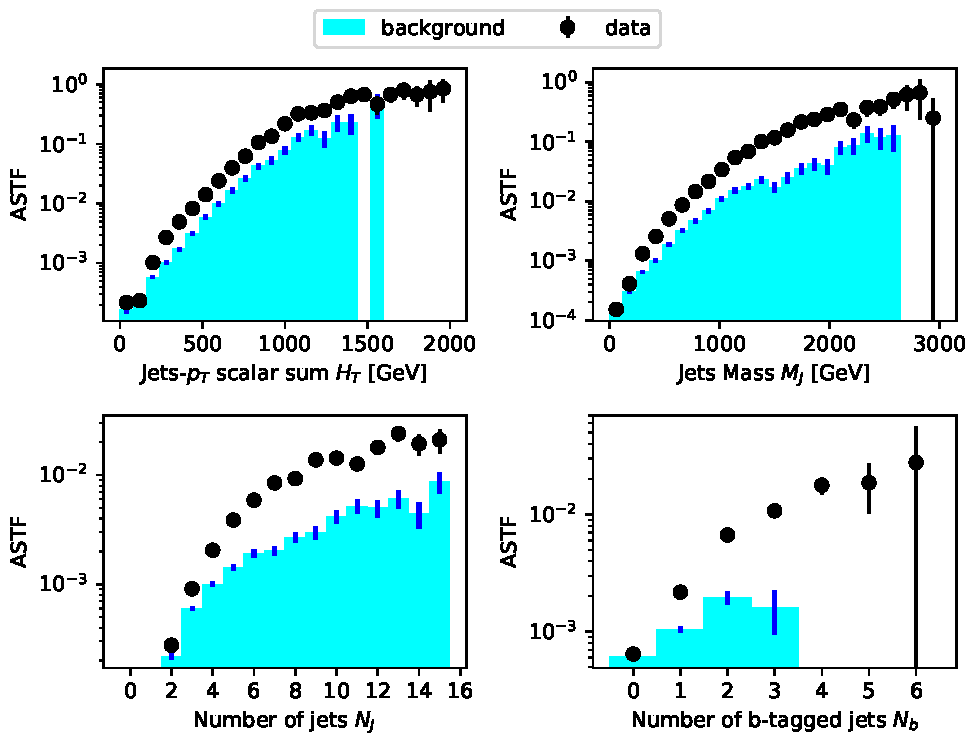
\includegraphics[width=0.7\textwidth]{astf.pdf}
\end{center}

\begin{itemize}
    \item<1-> Idea: select events where $\text{ASTF}(q)_{\text{data}} \gg \text{ASTF}(q)_{\text{background}}$
    \item<2-> Fulfilled for events in the bins $N_J\geq 6$ and $N_b\geq 2$
    \item<3-> Looking for a process that produces many high energy jets, some of which originating from b quarks.
\end{itemize}
\end{frame}

\begin{frame}{Postselection result}
\begin{center}
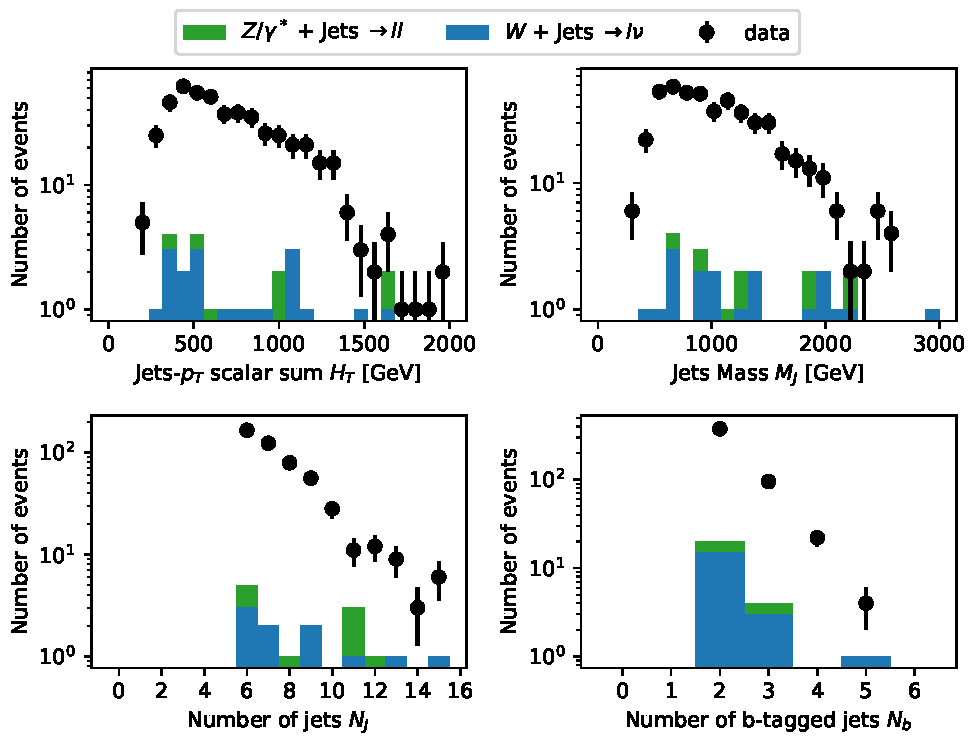
\includegraphics[width=0.7\textwidth]{post_b.pdf}
\end{center}

\begin{itemize}
    \item<1-> Almost all background events have vanished
    \item<2-> $\implies$ Remaining events in data must stem from a missing process (signal)
\end{itemize}
\end{frame}

\begin{frame}{Discussion}
\begin{itemize}
    \item<1-> At no point did we specify any property of the signal. Yet we were able to obtain an almost pure sample of signal events.
    \item<2-> Next step: Release samples in a dedicated dataset
    \item<3-> Theorists can study those events (e.g. with visual inspection or studies of reconstructed objects)
    \item<4-> Finally, this process would lead to a proposal for an extension of the SM to explain the signal
\end{itemize}
\end{frame}

\subsection{Verification of the discovery}
\begin{frame}{Overview}
\begin{itemize}
    \item<1-> Go back to present where the properties of the top quark are well understood
    \item<2-> Theory predicts:
    \begin{itemize}
        \item<3-> $pp \rightarrow t\bar{t}$ with $\sigma_{t\bar{t}}=164\,\textup{pb}$ at $\sqrt{s}=8\,\textup{TeV}$ (LO)
        \item<4-> Top quark decays before it can form hadrons
        \item<5-> Decays almost exclusively in $t \rightarrow W^+ b$ (due to $V_{tb}=0.999$)
        \item<6-> Overall: $t \rightarrow W^+ b \rightarrow W^+ + \textup{b-Jet} \implies$ high number of b-tagged jets 
        \item<7-> Single top quark production ($\sigma_{t}=87.7 \pm 5.8 \, \textup{pb}$ at $\sqrt{s}=8\,\textup{TeV}$) is removed by postselection with $N_b\geq 2$
    \end{itemize}
    
    \item<8-> We add $pp \rightarrow t\bar{t}$ to the background to see if this can explain the miss match.
\end{itemize}
\end{frame}

\begin{frame}{Distributions including the top quark}
\begin{center}
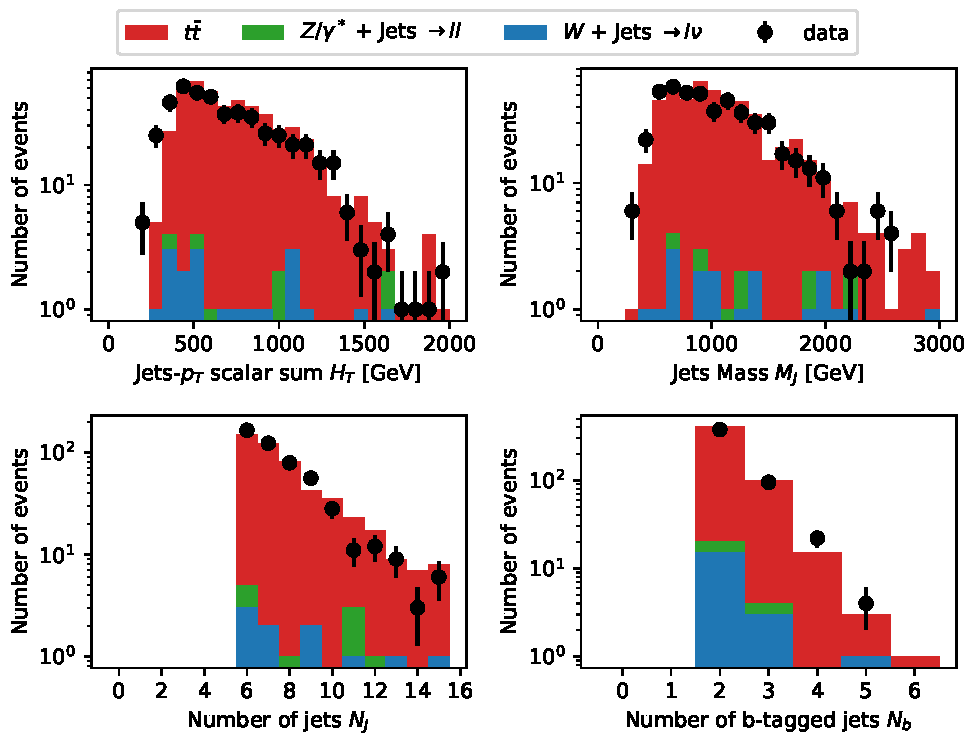
\includegraphics[width=0.8\textwidth]{post_tt.pdf}
\end{center}

\begin{itemize}
    \item<1-> Background + $t\bar{t}$ agrees closely with data
\end{itemize}
\end{frame}

\subsection{Discussion}
\begin{frame}{Distributions including the top quark}
\begin{center}
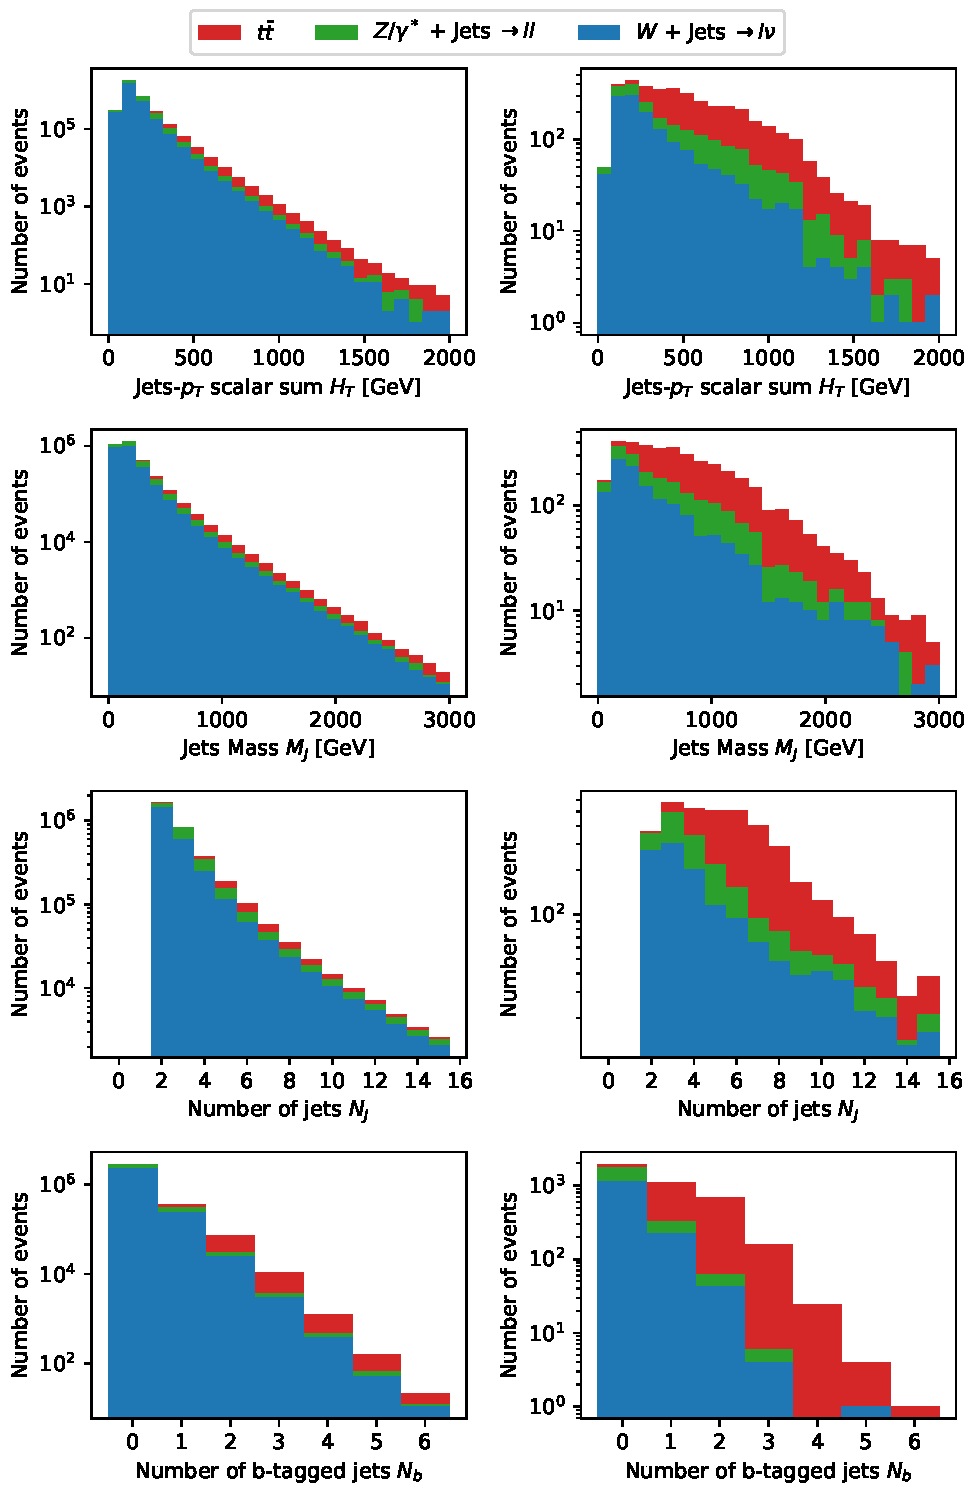
\includegraphics[width=0.5\textwidth]{mc_tt.pdf}
\end{center}
\end{frame}

\begin{frame}{ROC and $\textup{LR}_+$ for $t\bar{t}$}
\begin{center}
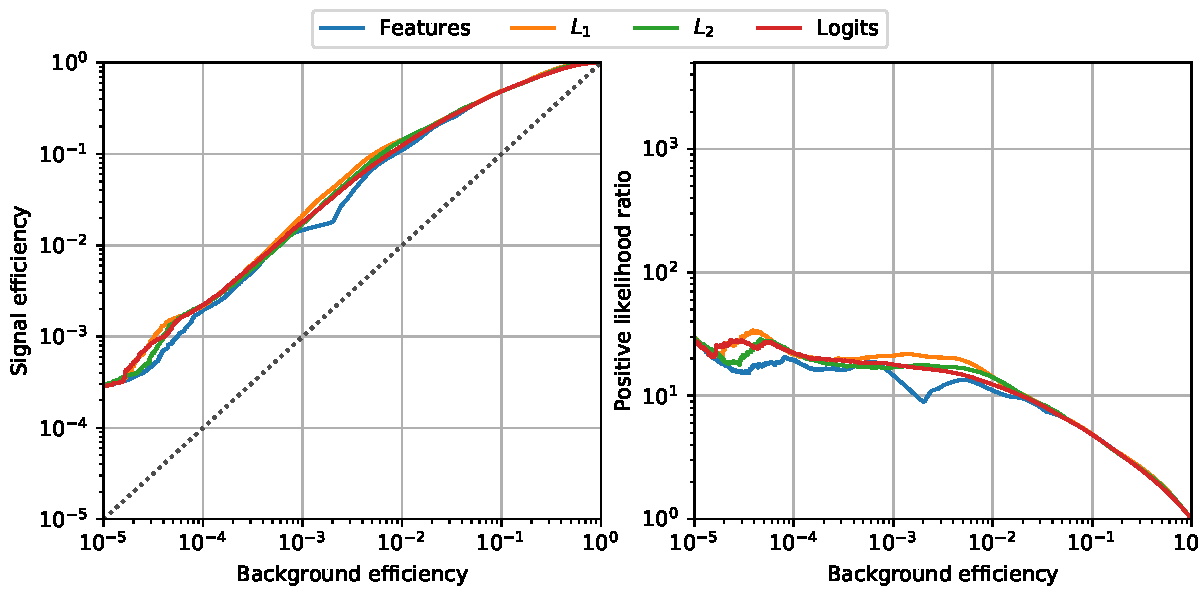
\includegraphics[width=0.8\textwidth]{roc-tt.pdf}
\end{center}
\begin{itemize}
    \item<1-> Working point set at $O(10^{-3}) \implies \textup{LR}_+ \sim 20$ 
    \item<2-> Low $\textup{LR}_+$ probably due to relatively high abundance of $t\bar{t}$
\end{itemize}
\end{frame}

\begin{frame}{Discussion}

\begin{itemize}
    \item<1-> Extracted preliminary properties of $t\bar{t}$ events with anomaly selection
    \item<2-> Obtained an almost pure sample of $t\bar{t}$ events by analyzing the ASTF
    \item<3-> No assumptions were made about this process $\implies$ achieved model-independent offline analysis
    \item<4-> Admittedly, we were lucky to already consider $N_J$ and $N_b$, which were crucial for the analysis and had the property $\text{ASTF}(q)_{\text{data}} \gg \text{ASTF}(q)_{\text{background}}$
    \item<5-> In practice: Compute ASTF for all possible quantities until one finds a quantity satisfying $\text{ASTF}(q)_{\text{data}} \gg \text{ASTF}(q)_{\text{background}}$
\end{itemize}
\end{frame}


\section{Conclusion}
\begin{frame}{Conclusion}
  \begin{itemize}
  \item<1-> We studied ALAD as an alternative to VAE
  \item<2-> Benchmark: ALAD is at least comparable to VAE
  \item<3-> ALAD is more flexible than VAE (no modifications needed for different scenarios) $\implies$ can run grid search on possible input quantities
  \item<4-> We presented an offline-analysis strategy and demonstrated its effectiveness
  \item<5-> We believe such a strategy could prove fruitful in the current and next phase of the LHC
  \end{itemize}
\end{frame}

\end{document}


